\scanpage{53}
explication ``à priori'' de l'\deleted{construction de} \inserted{invariance} affirmée par Washnitzer-Monsky.
C'est bien vrai si $S$ est de car. zéro, mais malheureusement c'est faux en car $p>0$, $\overline{\mathrm m}$ si on considère pour $f$ des projections structurales de \inserted{familles de} courbes elliptiques (= \unsure{schém.} elliptiques)!
\unsure{Il} s'agit donc pour le moment d'une relation heuristique et sentimentale, entre deux idées différentes, dont les relations exactes restent \deleted{\unsure{pour}} \inserted{loin} encore \inserted{d'avoir} été bien élucidées .....

\figure{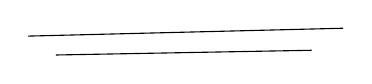
\begin{tikzpicture}
\draw (0,0)--(4.0,0.1);
\draw (0.35,-0.24)--(3.6,-0.18);
\end{tikzpicture}}

Pour résumer, on se trouve \unsure{actuellement} devant un puzzle, où il s'agit de reconstituer une théorie d'ensemble \deleted{\unsure{tenant compte}} \deleted{et} combinant

a) Une théorie cohomologique des complexes d'opérateurs différentiels, \deleted{qui} (notamment en vue d'application aux complexes de DR)

b) Une étude systématique des structures stratifiées, notamment \inserted{\unsure{mod. cohérents ou espaces fibrés}} \unsure{celles} qui \unsure{s'introduisent|à titre dérivé}

c) La théorie de Washnitzer-Monsky.

\margin{52}
